\documentclass{article}
\usepackage[utf8]{inputenc}
\usepackage{graphicx}
\usepackage{mathtools}
\usepackage{amssymb}
\usepackage{amsmath}
\usepackage{macros}
\usepackage{color}

\begin{document}

\section{TATA41 - Derivata}
Har vi stött på i gymnasiet. Kommer från Newton och Libnitz. Ur Newtons studie i mekanik.
Hastighet, rörelse per en tidsenhet. Medelhastigheten är helt enkelt sträckan genom tiden.
Om man låter tidsintervallet bli kortare och kortare så kommer man närmare och närmare derivatan.

\subsection{Definition}
Antag att funktionen $f$ är definierad i em omgivning av $a\in\R$. Då säges $f$ vara derivervar i punkten a,
med derivatan A, ifall gränsvärdet
$$ A = \lm h \infty \f{f(a+h)-f(a)}h = \lm x a \f{f(x)-f(a)}{x-a} $$
existerar (ändligt).\\
Derivatan betecknas $f'(a)$ eller $\dxf(a)$ eller $Df(x)$ eller\ldots
%\img{img\iphone_derv1.png}

\subsection{Anmärkning}
Sv: derivata,
Eng: derivative\\
Sv: att derivera,
Eng: to differentiate\\
Sv: att härleda,
Eng: derive

\subsection{Sats}
Om $f$ är deriverbar i punkten a så är $f$ kontinuerlig där.

\subsection{Bevis}
$$ f(x)-f(a) = (x-a) \times \f{f(x)-f(a)}{x-a} \to 0 \times f'(a) = 0, x \to a, f(x)\to f(a) $$

\subsection{Anmärkning}
Kontinuitet är alltså ett nödvändigt villkår för deriverbarhet, men det är inte ett tillräckligt villkor
vilket följande exempel visar.

\subsection{Exempel}
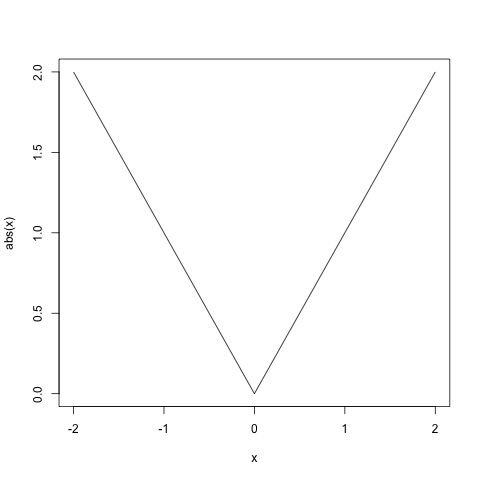
\includegraphics[height=60mm, width=60mm]{img/abs.png}
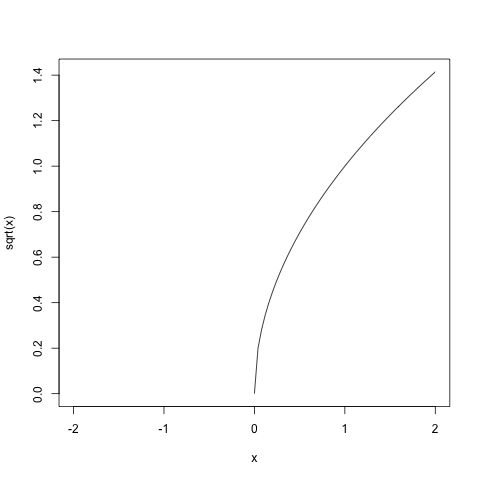
\includegraphics[height=60mm, width=60mm]{img/sqrt.png}
$y=f(x)=\abs x$ är kontinuerlig (överallt) men inte deriverbar i punkten $x = 0$.
Höger respektive vänstergränsvärde till derivatans gränsvärde är olika, alltså existerar ej derivatan
(dock så existerar höger respektive vänster derivatan).
Det finns funktioner som är kontinuerlig men inte deriverbar i någon punkt. (se Weierstrass 1872).

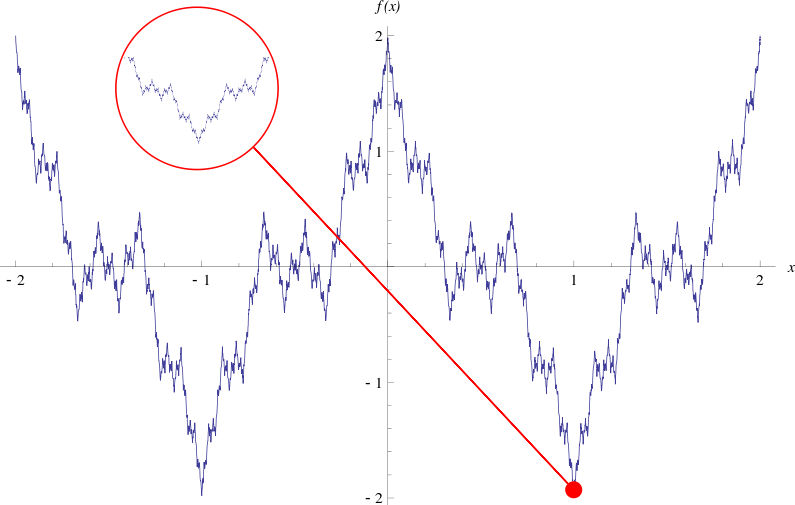
\includegraphics[height=60mm, width=120mm]{img/WeierstrassFunction.png}
\subsubsection{Krav}
Mängden av alla deriverbara funktioner är en äkta delmängd av alla kontinuerliga funktioner.
Deriverbarhet är alltså ett starkare krav än kontinuitet.

\subsection{Exempel (Konstant funktion)}
$ f(x) = c $ ger
$$ \f{f(x+h)-f(x)}h = \f{c-c}h = 0 \to 0, h \to 0; f'(x) = 0, \all x. $$

\subsection{Exempel (Monoma funktioner)}
$ f(x) = x^4 $ ger 
$$ \f{f(x+h)-f(x)}h = \f{(x+h)^4 - x^4}h = \f{(1x^4 + 4x^3h^1 + 6x^2h^2+4x^1h^3+1x^0h^4)-x^4}h =$$
$$4x^3+(6x^2h + 4xh^2+h^3) \to 4x^3, h\to 0; f'(x) = 4x^3$$

Allmänt:
$$ f(x) = x^n \im f'(x) = nx^{n-1}, n\in\Z$$

Tillsammans med de lätt bevisade räknereglerna
$
\begin{cases}
(cf)' = cf',\\
(f+g)' = f' + g'
\end{cases}
$
ger detta att vi kan derivera alla polynom, t.ex.
$$ \dx (x^3+5x^2+7x+43) = 3x^2+10x+7 $$

\subsection{Sats (produktregeln)}
Om $f$ och $g$ är deriverbara så är
$$ (fg)' = f'g + fg' $$

\subsection{Bevis (produktregeln)}
Med F=fg har vi
$$ \f{F(x)-F(a)}{x-a} = \f{f(x)g(x) - f(a)g(a)}{x-a} = $$
$$ \f{f(x)g(x) - f(a)g(x) + f(a)g(a) - f(a)g(a)}{x-a}  = $$
$$ \f{f(x)-f(a)}{x-a}g(x) + f(a)\f{g(x)-g(a)}{x-a} \to f'(a)g(a)+f(a)g(a), x\to a $$

\subsection{Exempel}
Låt $n>0$. För $x\neq 0$ gäller $x^nx^{-n}=1$\\
Derivera ger
$0 = (1)' = (x^nx^{-n})' = (x^n)'x^{-n} + x^n(x{-n})'
= nx^x{n-1}x^{-n} + x^n(x{-n})' \im (x^{-n})' = -nx^{-n-1}$

Regeln $(x^m)' = mx^{m-1}$ gäller alltså för alla heltal (inte bara positiva).
T.ex. $$D(\f 1x) = D(x^-1) = -1x^{-2} = \f{-1}{x^2}$$

\subsection{Exempel}
$ f(x)=e^x (= \exp x) $ ger
$$ \ddef fxh = \f{e^{x+h} - e^x}h = \f{e^xe^h - e^x}h = e^x\f{e^h-1}h \to e^x, h\to 0 $$
dvs $f'(x) = e^x$\\
Kort uttryckt $D\exp = \exp$

\subsubsection{Andra standardgränsvärden ger (se boken)}
$$ D\sin = \cos $$
$$ D\cos = -\sin $$
samt $\dx(\ln{\abs x}) = \f 1x, (x\neq 0)$

\subsection{Sats (Kedjeregeln)}
Om $f$ och $g$ är derivervara så är
$$ (f\circ g)' = (f'\circ g)g' $$
Med $y=f(t)$ och $t=g(x)$ kan man skriva kedjeregeln som
$$ \dxy = \f{dy}{dt} \f{dt}{dx} $$
där det är underförstått i vilka punkter som derivatorna ska beräknas

\subsection{Bevis (Kedjeregeln)}
Se boken.

\subsection{Exempel}
$$ D(\sin(x^5)) = \cos(x^5) \times 5x^4 $$

\subsection{Sats (Kvotregeln)}
Om $f$ och $g$ är derivervara så är
$$ (\f fg)' = \f{f'g-fg'}{g^2}, g\neq 0 $$

\subsection{Bevis (Kvotregeln)}
$$ (\f fg)' = (f\times g^{-1})' = f' \times \f 1g + f\times (\f 1g)' =
\f{f'}g + f\times \f{-1}{g^2}\times g' = \f{f'g-fg'}{g^2}$$

\subsection{Exempel}
$$D(\tan x) = D(\f{\sin x}{\cos x}) = \f{D(\sin x)\cos x - \sin x D(\cos x)}{\cos^2 x} =$$
$$\f{\cos x\cos x-\sin x\times (-\sin x)}{\cos^2 x} =
\f{\cos^2 x + \sin^2 x}{\cos^2 x} = \f 1{\cos^2 x}$$

\subsection{Sats (Derivatan av invers)}
Antag att $f$ är en inverterbar, kontinuerlig funktion som är deriverbar i punkten a. Om $f'(a)\neq 0$
så är $f^{-1}$ deriverbar i punkten $b=f(a)$ med derivatan $(f^{-1})'(b) = \f 1{f'(a)}$

\subsection{Bevis/rimliggörande}
Se boken.

\subsection{Exempel}
Vi såg tidigare att $f(x)=\tan x$ har derivatan $f'(x)=1+\tan^2 x$\\
Med $b=f(a)=\tan a, a\in ]-\f \pi 2, \f \pi 2[$ fås alltså
$ f'(a) = 1+\tan^2 a = 1+b^2$, så
$$ (f^{-1})'(b) = \f 1{f'(a)} = \f 1{1+\tan^2 a} = \f 1{1+b^2}$$
Med andra ord:
$$ \dx(\arctan x) = \f 1{1+x^2}$$

\end{document}
